\section{Authoring Interface}
\subsection{Key Features} Motivated by these insights, we developed the \systemname\  interface to support a dynamic workflow for script writing and  audio recording/editing. Our interface is built on two key features. 

\begin{figure*}
  \centering
  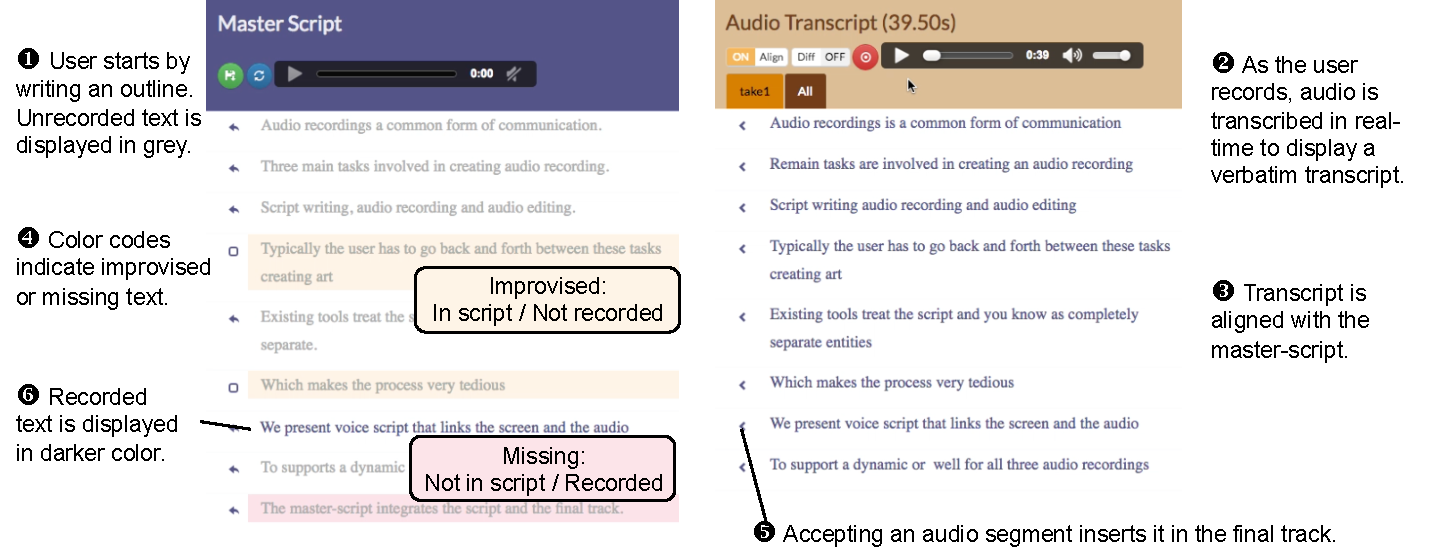
\includegraphics[width=2.0\columnwidth]{figures/ui_aligned}
  \caption{The \systemname\ interface. }~\label{fig:ui_aligned}
\end{figure*}

\textbf{Text-based representation of audio.} Previous work~\cite{casares2002simplifying,whittaker2004semantic,berthouzoz2012tools,rubin2013content} have shown that text-based representation of audio greatly facilitates navigation and editing. Moreover, since scripts are also composed in text, a text view of the audio  helps to link and unify the script
with the audio.
 Our system uses automatic speech recognition to transcribe the audio recordings in realtime, and represent each take with a\ verbatim transcript. The final track, composed from these takes, is also represented as text. Hence, the task of editing and combining the audio recordings becomes akin to merging text documents. 

\textbf{Master-script linking script and audio.} Unlike existing tools, our interface does not make a distinction between the script and the final audio track. Instead, our interface includes a \textit{master-script} document that represents both the script (i.e. what the user planned to record) and the transcript of the final track (i.e. what the user actually recorded). The master-script evolves throughout the authoring process, as the user records new takes and merge parts of it in, adds or deletes text to be recorded, or edits recorded text. 

% As shown in Figure~\ref{interface}, our interface consists of two types of documents: a \textit{Master Script} document (left) displays the current status of the final track, including what has been recorded and what was planned to be recorded but has not been recorded yet (i.e. the original script), while a \textit{Transcript} document (right) displays the verbatim transcript of individual audio takes. As the user records new takes, our tool aligns the audio transcripts to the master script so that it is easy to compare each take with the master script and with each other. It also partitions each recording into segments that can be seamlessly joined between takes. At any point during the recording process, the user can edit the script or the final track by editing the master script like a text document.

\subsection{Interface and Usage Scenario}
The rest of the section describes the interface using an example scenario of how a user might create an audio recording from the beginning. 

Typically the user begins by writing on the master-script an outline  of points to record. The text appears in light grey to indicate that these parts have not been recorded yet. At this stage, the master-script is like an ordinary
word document or script. 

Once the user starts recording, the audio is transcribed in real time and a verbatim text corresponding to each take appears in a separate transcript document tab. Each transcript is time-aligned with the corresponding recording, so the user can quickly navigate to specific
part of the audio by clicking on a word in the transcript. If the \textit{diff-view} is on, the per-word difference between the transcript and the master-script text is displayed like \textit{track change markers} in word processing tools. That is, missing words are crossed out and extra words are highlighted. If the \textit{compare-view} is on, our system aligns segments of the transcript to corresponding segments in the master-script, (in this case the points in the original outline), and shows them side-by-side (Figure~\ref{fig:ui_aligned}). A segment in the transcript that does not correspond to any part of the master-script (e.g. where the speaker improvised)is highlighted in yellow.

% partitions the transcript and the master script into short segments, and aligns them to each other. The boundaries of these segments are computed by taking into account, along with other factors,  pauses in the audio, such that when different audio segments corresponding to the transcript segments are joined together the cut is seamless.

The user can \textit{accept} an audio segment into the final track
by clicking on a button next to each transcript segment. If there was
a corresponding  segment in the master-script, the transcript segment
replaces it. If the audio was improvised the transcript segment
is simply inserted into the master-script.
The text of the accepted segment appears in
darker color in the master-script to indicate that it has been recorded. 

After the user records multiple takes, in addition to each of the transcripts, the \textit{all tab} provides a summary of all of the takes. For each segment in the master script, it displays corresponding transcript segments, this time from all of the audio takes. A drop-down button next to a transcript segment  indicates that there are multiple versions (or takes)  of the  segment. Clicking on the button opens a
list showing the alternative versions (Figure ~\ref{alternate-view}) \VTODO{capture of dropdown showing alternate takes}. The user can listen to any of these takes and select one without having to search through individual takes. 

If a part of the master-script has not been recorded in any of the takes, it is highlighted in red. In this way, the user can easily keep track of what has been already recorded, and what still needs to be recorded. After recording and accepting segments to the final track, the master-script contains both recorded and unrecorded text.
The final track includes only the darker, recorded text. 

 During any point in the process, the user can edit the master-script like a text document.
For example, the user can simply insert
more text to record (which appears in light grey), or make changes
to unrecorded text to flesh out the original outline
or change the wording of a particular sentence. If the user deletes a recorded word from the text, it will be deleted from the final track. The user can also correct the transcription of a recorded word without affecting the underlying audio. When the user edits a recorded word (without completely deleting it), the word is italicized and marked red to warn the user that it may no longer match the underlying audio. If the edit was made to correction a transcription error and the word does indeed match the audio, the user can manually mark the word as \textit{clean} which returns it to a normal dark font. If the edit was intended to change the content, the user can use the mark as a reminder to re-record that portion of the audio.

   

In order to produce the final recording, the user iterates back and forth between all of these operations, editing the master-script, recording audio takes, comparing alternative takes and accepting audio segments into the final track.
The beauty of our interface is that it supports a wide range of workflows for different users and scenarios. For instance, instead of starting with a written outline, the user can begin with an empty master-script and simply start recording,  then use  the initial recording as an outline. The user can also record the entire script in a single take, or work on a single section at a time. 
